\chapter{Monte Carlo Compartmental Method}
\label{chap2}

\hspace{\parindent} Modelling epidemics has been done in order to study the mechanisms by which diseases spread. This helps in predicting how fast and far the disease can spread in order to control and prevent future outbreaks \cite{Arino453}. By treating the applause similarly to a disease that spreads in the audience, the same tools to model epidemics can be used to model the applause \cite{Mann20130466}. 

\section{Compartmental Model}
\subsection{States}

\hspace{\parindent}The proposed compartmental model separates the agents into two states, silent (S) and clapping (C). 
The silent state replaces the susceptible state while clapping state replaces the infected state. 
Intuitively, agents in state S are audience members who are not clapping while agents in state C are audience members who are clapping.
The number of agents in state S, given by $n_{s}$, and the number of agents in state C, given by $n_{c}$, dictate the state of the system, given by $\vec{n}$ where $\vec{n}\equiv(n_{c},n_{s})$.
It is assumed that the total number of agents $N$ is fixed, where $N = n_{c} + n_{s}$ and $\vec{n}$ is fully specified by $n_{c}$ alone.

\begin{figure}
 \centering
  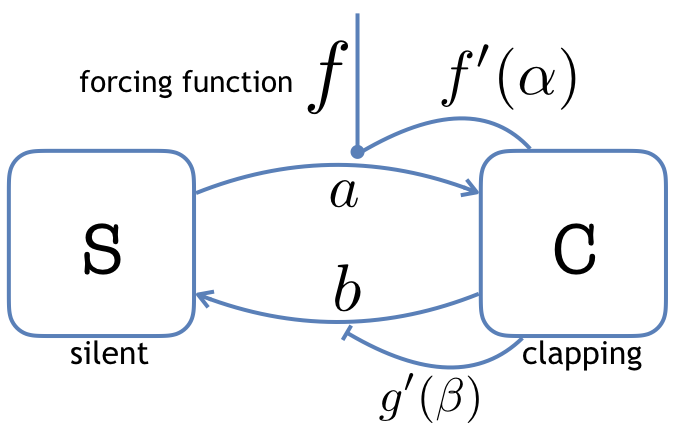
\includegraphics[width=0.5\linewidth]{images/chapter2/model2.png}
  \caption{The compartmental model of audience applause based on the SIS epidemic model. Agents are either in state S or state C. Parameters $a$ and $b$ are the transitional probabilities. Functions $f$, $f'$, and $g'$ are further discussed.}
  \label{fig:SCSmodel}
\end{figure}

\subsection{Parameters}
\hspace{\parindent}The parameters $a$ and $b$ are the transition parameters.
They range from $0$ to $1$ to represent transitional probabilities.
The transitional probabilities from S to C and C to S are controlled by $a$ and $b$ respectively.
The corresponding transition probabilities are given by ${R}_{1}$ and ${R}_{2}$ where
\begin{eqnarray}
\mathrm{R}_{1} &:& \mathrm{S} \overset{a}{\longrightarrow} \mathrm{C} \label{eq:r1} \\
\mathrm{R}_{2} &:& \mathrm{C} \overset{b}{\longrightarrow} \mathrm{S}.\label{eq:r2}
\end{eqnarray}


\subsection{Functions}
\hspace{\parindent}An audience is initially silent until given a social cue to start clapping, such as the end of a performance. 
This corresponds in the model to all agents starting in state S, and then forcing the agents to undergo $\mathrm{R}_{1}$.
The function $f$ forces the transition ${R}_{1}$ for an indicated time interval, $\tau$, which is typically 2-3 seconds/iterations.
Once $f$ expires, the system behaves freely and its agents may undergo various $\mathrm{R}_{1}$ and/or $\mathrm{R}_{2}$ transitions depending on the given parameters.


Aside from social cues, audience members may start clapping simply because others are.
The peer influence may cause agents unaffected by social cues to start clapping, or those who have already stopped clapping to clap again.
This creates a feedback mechanism that initiates more people to clap if majority of the agents are clapping corresponding in the model to the function $f'$.
The function $f'$ incorporates this feedback mechanism and is parametrized by $\alpha$:
\begin{equation}\label{eq:f'}
  f'(\alpha) = \alpha \frac{n_c}{N-1},
\end{equation}
where $\alpha$ ranges from $0$ to $1$ for probabilistic interpretations.
The probability for a spontaneous $\mathrm{R}_{1}$ transition is directly proportional to $\alpha$ and the fraction of the population in state C. 
The denominator is set to $N-1$ because an agent cannot spontaneously influence itself; it is only influenced by the rest of the population.
The function is more effective when there are more agents in state C.

Finally, audience members may contain their own bias towards a social event and may applaud longer or shorter depending on the bias.
Also, the continuous applause of the majority can inhibit those who are clapping to stop clapping.
This corresponds in the model to the function $g'$.
The factor $g'$ incorporates the inhibition as a modulation function and is parametrized by $\beta$: 
\begin{equation}\label{eq:g'}
  g'(\beta) = \frac{1}{1 + \beta\;n_C /(N-1)}
\end{equation}
where $\beta \geq 0$, representing the bias.
Higher $\beta$ translates to agents less likely to undergo transition $\mathrm{R}_{2}$ 
Equation (\eqref{g'}) is taken from the Michaelis-Menten equation, which aims to model enzyme kinetics\cite{michaelisconstant}.

This completes the differential equations for the reactions \eqref{eq:r1} and \eqref{eq:r2}:
\begin{eqnarray}
\frac{d}{dt}n_{c} &=& a (f+f'-f'f) n_{s} - b g' n_{c}\label{eq:diff1} \\
\frac{d}{dt}n_{s} &=& b g' n_{c} - a (f+f'-f'f) n_{s}\label{eq:diff2}
\end{eqnarray}
These equations are consistent with the assumption that the total audience size is fixed, that is $dn_{c}/dt = -dn_{s}/dt$.
The derivation for the combined probability of the functions f and f' is shown in Appendix \ref{apndx:prob}.



\section{Simulation Alogrithm}
\hspace{\parindent} The compartmental SIS-like model is confirmed by simulating the $\mathrm{R}_{1}$ and $\mathrm{R}_{2}$ process via an agent-based Monte Carlo method. For each iteration, every agent is assigned a random number that is compared to one of the transition probabilities:

\begin{eqnarray}
P(\mathrm{R}_{1}) &&= a(f + f' - f'f) \label{eq:p(r1)} \\
P(\mathrm{R}_{2}) &&= bg' \label{eq:p(r2)}
\end{eqnarray}

Agents in state S undergo transition $\mathrm{R}_{1}$ with probability shown in \ref{eq:p(r1)}.
Agents in state C undergo transition $\mathrm{R}_{2}$ with probability shown in \ref{eq:p(r2)}.
A uniform random number, $u$, where $u \in [0,1]$, is drawn from a random number generator and then compared to the corresponding probability $P$.
If $u \leq P$, the appropriate transition is allowed to occur.
%The code developed to simulate the audience applause is provided in Appendix \ref{apndx:codelib}.

\dimendef\prevdepth=0
\begin{figure}[h!]
  \centering
  \begin{subfigure}[b]{0.4\linewidth}
    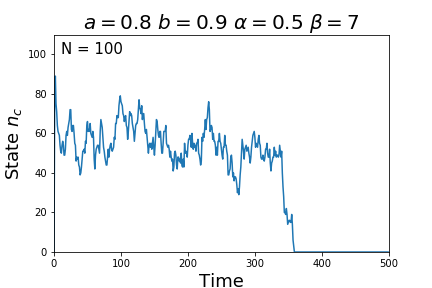
\includegraphics[width=\linewidth]{images/chapter2/simA.png}
    \caption{A simulation with finite applause time.}
  \end{subfigure}
  \begin{subfigure}[b]{0.4\linewidth}
    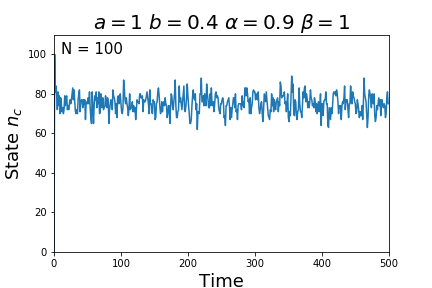
\includegraphics[width=\linewidth]{images/chapter2/simB.png}
    %\label{fig:nonTrivSim}
    \caption{A simulation that seams to oscillate in a certain value.}
  \end{subfigure}
  \caption{Sample simulations given a fixed population $N = 100$. Simulation (a) is a typical, intuitive audience applause that has an end. Simulation (b) is non-trivial and counter-intuitive in that it seems to have no end.}
  \label{fig:simulations}
\end{figure}




The simulator outputs a graph of $n_{c}$ versus time, where time is defined to be each iteration.
Examples of such simulations are shown in figure \ref{fig:simulations}.
An emergent property of the system is that a certain set of parameters will simulate an audience applause that does not end.
Even if such cases do not exist in real life, further investigation of the steady-state applause may unravel the complexity of the system.


